\documentclass[a4paper,10pt]{scrartcl}
\usepackage[utf8]{inputenc}
\usepackage[spanish]{babel} 
\usepackage[hidelinks]{hyperref}
\usepackage{color}
\usepackage{graphicx}
\graphicspath{ {images/} }


\title{Alcance del proyecto}
\subtitle{Grupo 1.2.2 - Redmine}
\author{
		Manuel Francisco López Ruiz\\
		Julio Márquez Castro\\
		Álvaro Martín Gordillo\\
		  }

\begin{document}

\clearpage\maketitle
\thispagestyle{empty}
\newpage

\tableofcontents

\newpage



\section{Objetivos del proyecto}

Obtener un alto nivel de conocimientos sobre la herramienta Redmine con el fin de ser capaces de transmitir los conocimientos aprendidos.

\section{Descripción del producto o servicio}

El servicio es un curso introductorio a Redmine donde se debe explicar que es, como se usa, errores comunes y ventajas e inconvenientes frente a otros servicios. Tras la explicación se realizará una práctica con el objetivo de que los asistentes puedan practicar los conceptos aprendidos y preguntar dudas.

\section{Requisitos del proyecto/producto}

\begin{itemize}
	\item Software Redmine
	\item Acceso a internet
	\item Servidor para Redmine
	\item Pc cliente
\end{itemize}

\section{Límites/restricciones del proyecto}

\begin{itemize}
	\item Limite de tiempo del vídeo tutorial
\end{itemize}

\section{Entregables}

El proyecto constará de un único entregable cuya fecha será el 7 de diciembre del año 2016 el cual contendrá:
	\begin{itemize}
		\item Un plan de gestión del trabajo el cual deberá incluir al menos:
		
		\begin{itemize}
			\item Acta de constitución.
			\item Definición del alcance.
			\item Planificación inicial y final.
			\item Lecciones aprendidas.
		\end{itemize}
		
		\item Un tutorial/vídeo destacando los aspectos más importantes del trabajo propuesto.
		
		\item Un enunciado de un ejemplo práctico con la resolución del mismo.
		
		\item La presentación de la exposición de la práctica que se realizará públicamente. Para ello, y a indicaciones del profesorado se podrá utilizar el tutorial/vídeo.		
	\end{itemize}

Así mismo se realizará una presentación del trabajo el 9 de diciembre del año 2016 con una duración máxima de 35 minutos constando de:
\begin{itemize}
	\item Descripción del trabajo realizado y lecciones aprendidas.
	
	\item Reproducción del vídeo de presentación global de la herramienta.
	
	\item Tutorial dirigido. \textbf{\textcolor{red}{¿¿¿¿¿Adicionalmente?????}} podrá constar de un ejercicio práctico para los asistentes a resolver en el tiempo disponible y aportar la solución del mismo.

	\item Preguntas.


\end{itemize}

\section{Criterios de aceptación}
El profesorado de la asignatura evaluará la calidad de los contenidos de la memoria y el tutorial/vídeo; la claridad de la exposición en la presentación y la adecuación del enunciado presentado.

\section{Exclusiones}
Será excluido en caso de que no se presente lo requerido en los entregables o que la calidad del contenido sea muy pobre e incompleta.


\section{Asunciones}

	\begin{enumerate}
		\item Podremos realizar toda la documentación necesaria con \LaTeX.
		\item Podremos aprender y trabajar con GIT\footnote{\url{https://git-scm.com/}}/GitHub\footnote{\url{https://github.com/}} sin ningún problema.
		\item Dispondremos de acceso a internet para poder usar las herramientas necesarias para el desarrollo.
	\end{enumerate}

\section{Riesgos iniciales}

Los riesgos iniciales encontrados son los siguientes:
\begin{enumerate}
	\item Desconocimiento por parte de parte del equipo de las herramientas usadas para el desarrollo de la documentación \LaTeX y GIT\footnote{\url{https://git-scm.com/}}/GitHub\footnote{\url{https://github.com/}}.
	
	\item Desconocimiento por todo el equipo de como realizar un vídeo tutorial.
	
	\item Desconocimiento parcial del uso para el que se debe realizar el tutorial (Redmine\footnote{\url{http://www.redmine.org/}}) puesto que ProjETSII\footnote{\url{https://projetsii.informatica.us.es/}} es una modificación del mismo pero no es igual.
\end{enumerate}


\section{Fechas importantes}
Las fechas importantes serán las siguientes:

	\begin{itemize}
		\item 28 de octubre del año 2016: Primera sesión de seguimiento del trabajo.
		
		\item 2 de diciembre del año 2016: Segunda sesión de seguimiento del trabajo.
		
		\item 7 de diciembre del año 2016: Entrega documentación y tutorial/vídeo.
		
		\item 9 de diciembre del año 2016: Presentación.
	\end{itemize}

\section{EDT}

	\begin{center}
		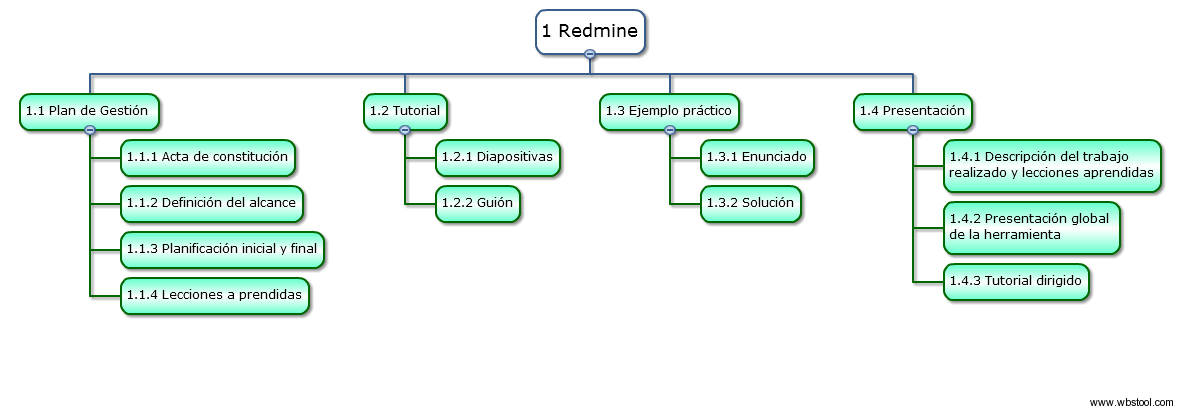
\includegraphics[width=\linewidth]{EDT}
	\end{center}

\section{Diccionario EDT}

\section{Estimación de costes}


\bibliography{sample}

\end{document}
